\documentclass[10pt]{beamer}

\usetheme{CambridgeUS}
\usepackage[english, russian]{babel}
\usepackage[utf8]{inputenc}
\usepackage{caption}
\usepackage{etoolbox}
\usepackage{multicol}
\usepackage{movie15}

\title[\href{https://goo.gl/NRgp8K}{https://goo.gl/NRgp8K} (Term 3)]{Вычислительная геометрия}
\author[Гусев Илья]{Гусев Илья}
\institute[МФТИ] 
{Московский физико-технический институт\\*}
\date{Москва, 2017}
\subject{Computer Science}

\begin{document}

\begin{frame}
  \titlepage
\end{frame}

\begin{frame}{Содержание}
\tableofcontents
\end{frame}

\section{Минимальная выпуклая оболочка}

\subsection{Что это?}
\begin{frame}[fragile]{Что это?}
\begin{enumerate}
\item Рассматриваем конечное множество точек на плоскости (2 координаты).
\item Оболочка множества точек - любая замкнутая кривая без самопересечений такая, что все точки из множества лежат внутри этой кривой.
\item Минимальная оболочка - оболочка минимальной длины (минимального периметра).
\end{enumerate}
\begin{center}
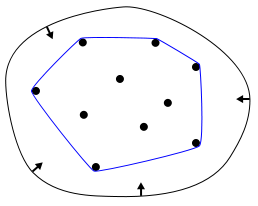
\includegraphics[width=5cm, height=4cm]{Term_3/Source/Pictures//convex1.png}
\end{center}
\end{frame}

\subsection{Скалярное и векторное произведение}
\begin{frame}[fragile]{Скалярное и векторное произведение}
\begin{enumerate}
    \begin{multicols}{2}
    \item Скалярное произведение:\\
        $\vec{a} \cdot \vec{b} = a_0 b_0 + a_1  b_1 $\\
        $\vec{a} \cdot \vec{b} = |a| |b| cos(\theta) $\\
        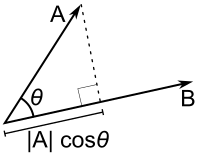
\includegraphics[width=3cm, height=2cm]{Term_3/Source/Pictures//scalar.png}
    \vfill\eject
    \item Векторное произведение: \\
        $|\vec{a} \times \vec{b}| = |a_0 b_1 - a_1 b_0 $\\
        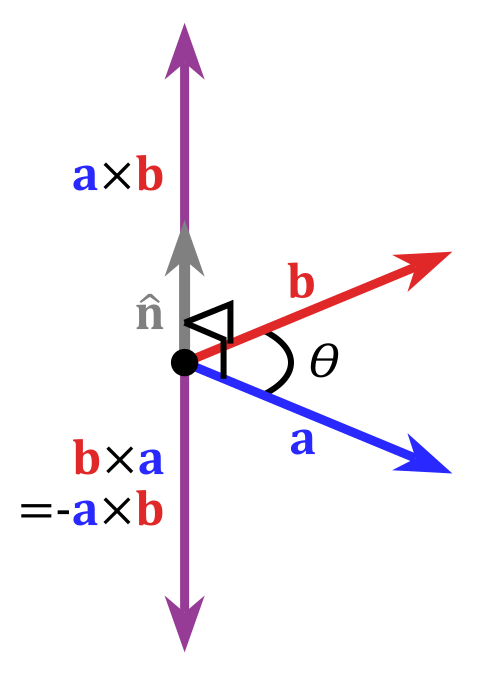
\includegraphics[width=2cm, height=3cm]{pictures/vector.png} 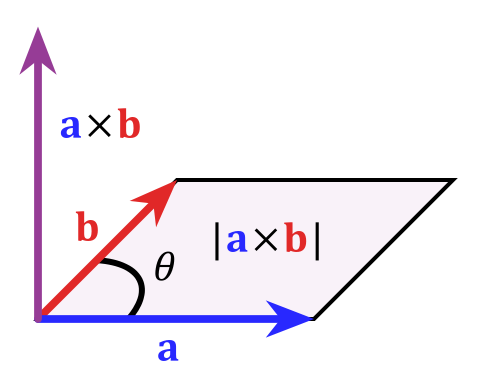
\includegraphics[width=3.5cm, height=3cm]{Term_3/Source/Pictures//vector2.png}\\
    \end{multicols}
\end{enumerate}
\end{frame}


\subsection{Алгоритм Джарвиса}
\begin{frame}[fragile]{Алгоритм Джарвиса}
\begin{enumerate}
\item Ищем выпуклую оболочку последовательно, против часовой стрелки, начиная с определенной точки.
\item Определённая точка - точно из оболочки, например самая нижняя.
\item На i-ом шаге рассматриваем все оставшиеся точки, и ещё $p_0$.
\item Ищется косинус угла через скалярное произведение между векторами $p_{i-1} p_i$ и $p_i p_{i+1}$, где $p_{i+1}$ - претендент на следующую точку оболочки.
\item Выбираем точку с максимальным косинусом (между векторами!).
\item Завершаем, когда снова натыкаемся на $p_0$. Сложность - $O(n*h)$.
\end{enumerate}
\begin{center}
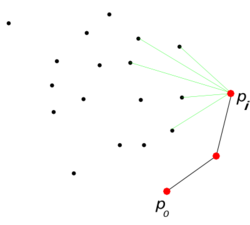
\includegraphics[width=5cm, height=4cm]{Term_3/Source/Pictures//jarvis.png}
\end{center}
\end{frame}

\subsection{Алгоритм Грэхема}
\begin{frame}[fragile]{Алгоритм Грэхема}
\begin{enumerate}
\item Берём самую нижнюю точку (например) и добавляем в ответ.
\item Сортируем все остальные точки по полярному углу относительно $p_0$.
\item Добавляем в ответ $p_1$ - самую первую из отсортированных точек.
\item Берем следующую по счету точку t. Пока t и две последних точки в текущей оболочке $p_i$ и $p_{i-1}$ образуют неправый поворот (вектора $p_i t$ и $p_{i-1} p_i$), удаляем из оболочки $p_i$.
\item Добавляем в оболочку t. Сложность - $O(n*log(n))$.
\end{enumerate}
\begin{center}
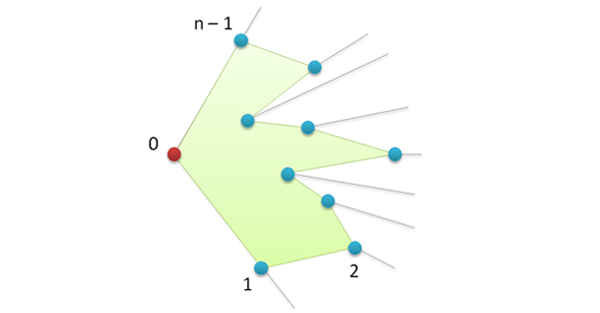
\includegraphics[width=7cm, height=4cm]{Term_3/Source/Pictures/graham2.png}
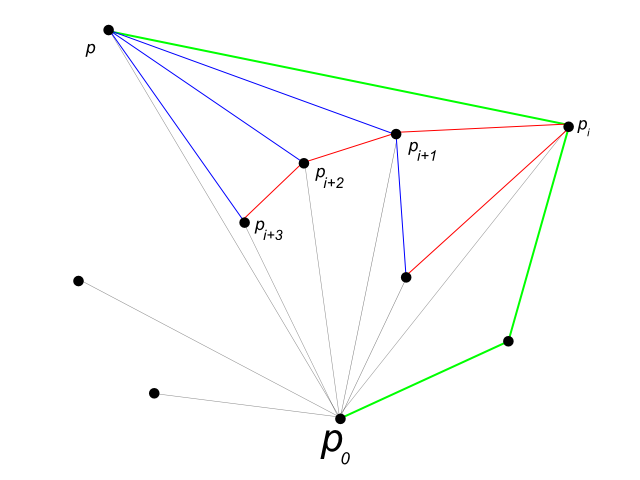
\includegraphics[width=5cm, height=4cm]{Term_3/Source/Pictures/graham.png}
\end{center}
\end{frame}

\subsection{Алгоритм Эндрю-Грэхема}
\begin{frame}[fragile]{Алгоритм Эндрю-Грэхема}
\begin{enumerate}
\item Находим самую левую и самую правую точки множества - $p_0$ и $p_1$.
\item Делим множество на две части: точки над и под прямой.
\item Для каждой половины ищем выпуклую оболочку Грехемом с условием, что сортируем не по полярному углу, а по координате.
\item Сливаем получившиеся оболочки.
\item Сложность - $O(n*log(n))$.
\end{enumerate}
\end{frame}

\subsection{Задача про диаметр}
\begin{frame}[fragile]{Суммы Минковского}
\begin{multicols}{2}
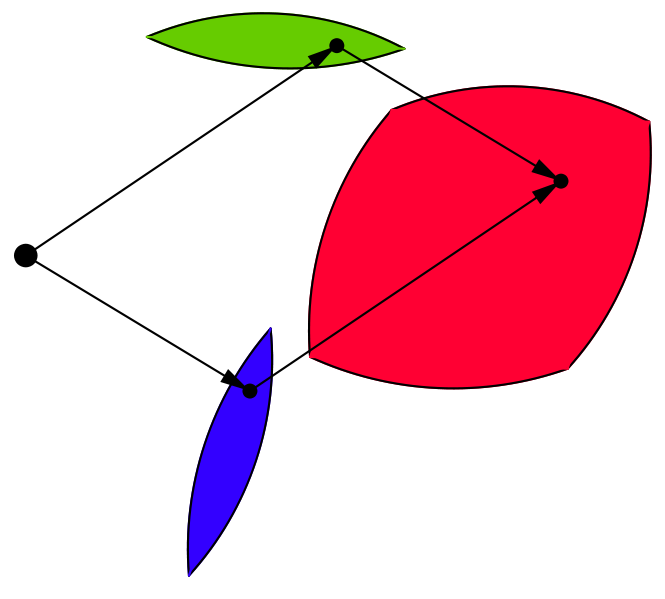
\includegraphics[width=6cm, height=5cm]{Term_3/Source/Pictures/minkovskii.png}
\vfill\eject
$C = \left\{\,c \mid c=a+b, a\in A, b\in B\,\right\}$\\
Красная фигура - сумма зеленой и синей
\end{multicols}
\end{frame}

\begin{frame}[fragile]{Задача про диаметр}
Поиск диаметра множества на плоскости за $O(n*log(n))$
\begin{enumerate}
    \item Строим выпуклую оболчку. (сложность - $O(n*log(n))$)
    \item Берём сумму Минковского выпуклой оболчки и минуса выпуклой оболочки ($\vec{a} \rightarrow -\vec{a}$). (сложность - $O(n)$)
    \item Выбираем максимум по модулю векторов всех вершин суммы Минковского. (сложность - $O(n)$)
\end{enumerate}
\end{frame}

\section{Другое}
\subsection{Нахождение пары ближайших точек}
\begin{frame}[fragile]{Нахождение пары ближайших точек}
\begin{multicols}{2}
"Разделяй-и-властвуй"
\begin{enumerate}
    \item Сортируем точки как пары чисел.
    \item Возьмём среднюю после сортировки точку $p_m (m = \lfloor n/2 \rfloor)$, и все точки до неё и саму $p_m$ отнесём к первой половине, а все точки после неё — ко второй половине.
    \item $h=\min (h_1, h_2)$, где h1 и h2 - с предыдущего уровня рекурсии, теперь - объединение.
\end{enumerate}
\vfill\eject
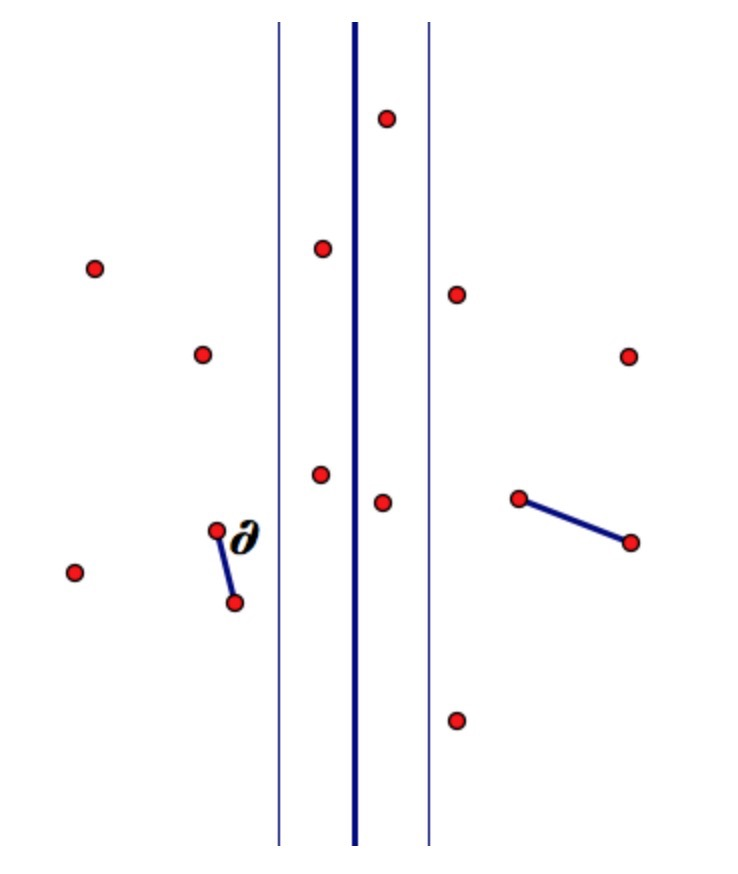
\includegraphics[width=5cm, height=6cm]{Term_3/Source/Pictures/geometry_points1.jpg}
\end{multicols}
\end{frame}

\begin{frame}[fragile]{Нахождение пары ближайших точек}
\begin{multicols}{2}
\begin{enumerate}
    \item $B = \{ p_i : | x_i - x_m | < h \}$. 
    \item $C(p_i) = \{ p_j : \ p_j \in B, y_i - h < y_j \}$
    \item Стадия объединения: построить B, отсортировать в нём точки по y-координате, затем для каждой точки $p_i \in B$ рассмотреть все точки $p_j \in C(p_i)$, и каждой пары $(p_i,p_j)$ посчитать расстояние и сравнить с текущим наилучшим расстоянием.
    \item $|C(p_i)| <= 8$
\end{enumerate}
\vfill\eject
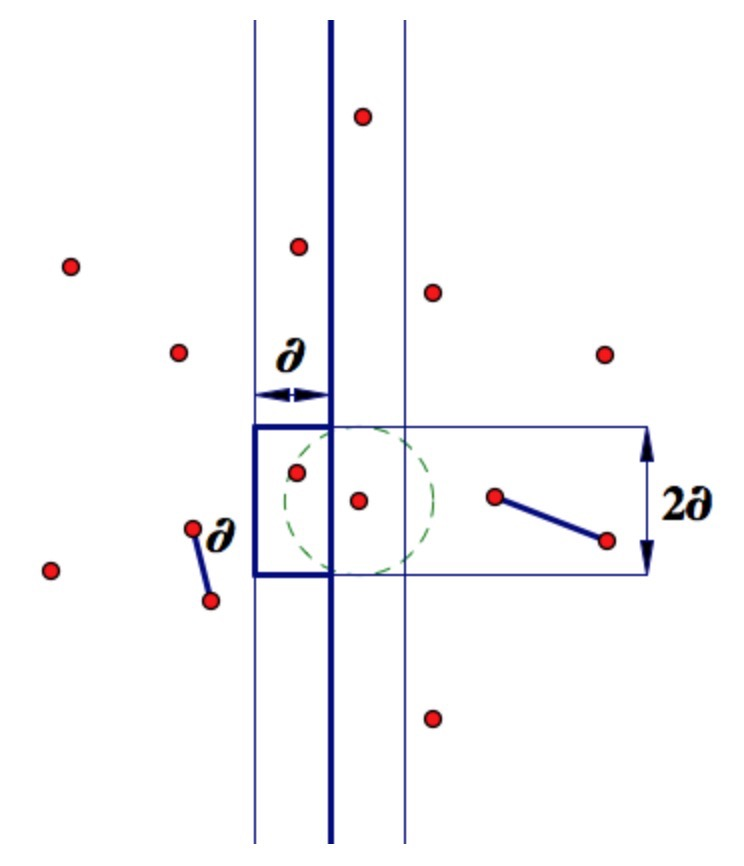
\includegraphics[width=5cm, height=6cm]{Term_3/Source/Pictures/geometry_points2.jpg}
\end{multicols}
\end{frame}


\appendix
\section<presentation>*{\appendixname}
\subsection<presentation>*{Useful links}

\begin{frame}[allowframebreaks]
  \frametitle<presentation>{Полезные ссылки}
    
  \begin{thebibliography}{10}
{
  \beamertemplatebookbibitems
  \bibitem{https://neerc.ifmo.ru}
  \texttt{https://neerc.ifmo.ru: выпуклые оболочки}
  \newblock \href{https://neerc.ifmo.ru/wiki/index.php?title=\%D0\%A1\%D1\%82\%D0\%B0\%D1\%82\%D0\%B8\%D1\%87\%D0\%B5\%D1\%81\%D0\%BA\%D0\%B8\%D0\%B5_\%D0\%B2\%D1\%8B\%D0\%BF\%D1\%83\%D0\%BA\%D0\%BB\%D1\%8B\%D0\%B5_\%D0\%BE\%D0\%B1\%D0\%BE\%D0\%BB\%D0\%BE\%D1\%87\%D0\%BA\%D0\%B8:_\%D0\%94\%D0\%B6\%D0\%B0\%D1\%80\%D0\%B2\%D0\%B8\%D1\%81,_\%D0\%93\%D1\%80\%D1\%8D\%D1\%85\%D0\%B5\%D0\%BC,_\%D0\%AD\%D0\%BD\%D0\%B4\%D1\%80\%D1\%8E,_\%D0\%A7\%D0\%B5\%D0\%BD,_QuickHull}{\texttt{https://neerc.ifmo.ru/wiki/index.php?title=Статические\\ \_выпуклые\_оболочки:\_Джарвис,\_Грэхем,\_Эндрю,\_Чен,\_QuickHull}}
  
  \bibitem{Habr: выпуклые оболочки}
  \texttt{Хабр: выпуклые оболчки}
  \newblock \href{https://habrahabr.ru/post/144921/}{\texttt{https://habrahabr.ru/post/144921/}}
  
  \bibitem{E-maxx: ближайшие точки}
   \texttt{E-maxx: ближайшие точки}
  \newblock \href{ https://e-maxx.ru/algo/nearest\_points}{\texttt{https://e-maxx.ru/algo/nearest\_points}}
 
}
    
  \end{thebibliography}
\end{frame}

\end{document}


